\section{选取特征进行实验}
\subsection{Matlab}
该部分进行的实验:用Matlab实现对浮游动物特征的提取(特征包括PkID中部分特征以及计算视觉中的一些特征提取方法),并进行分类。

选用特征Mean、StdDev、CV、SR、MeanPos、Elongation、Circ、Feret、PerimAreaexc、CDexc、Skelarea、FeretAreaexc、PerimFeret、矩形度、体态比、凸率、伸长度、灰度共生矩阵(对比度)、对称性(左右)。采用随机森林进行训练和分类得到的结果如图~\ref{fig:19-Features-MATLAB-our-RF},其分类准确率为72.9\%。采用SVM Linear进行训练和分类得到的结果如图~\ref{fig:19-Features-MATLAB-our-SVM-Linear},其分类准确率为58.9\%
\begin{figure}[!ht]
\centering
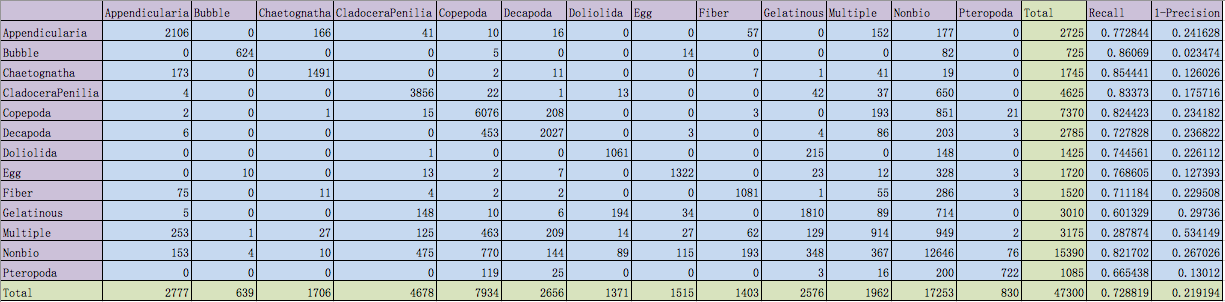
\includegraphics[width=1.0\linewidth]{19-Features-MATLAB-our-RF}
\caption{Matlab-19个特征采用随机森林进行分类的结果}
\label{fig:19-Features-MATLAB-our-RF}
\end{figure}

\begin{figure}[!ht]
\centering
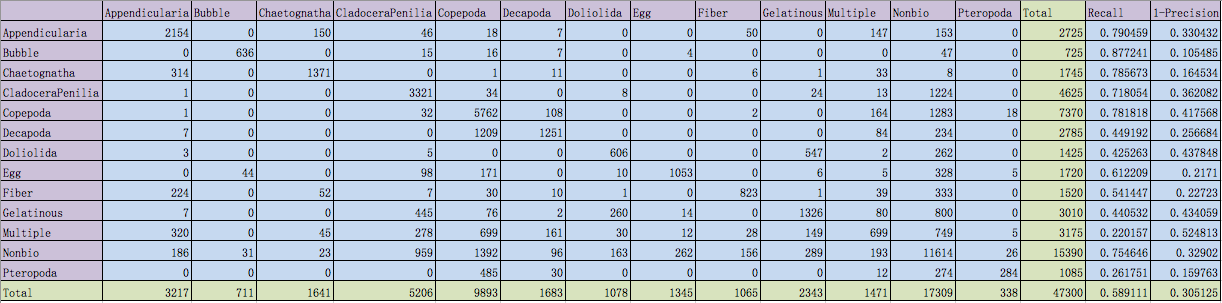
\includegraphics[width=1.0\linewidth]{19-Features-MATLAB-our-SVM-Linear}
\caption{Matlab-19个特征采用SVM Linear进行分类的结果}
\label{fig:19-Features-MATLAB-our-SVM-Linear}
\end{figure}